% GNUPLOT: LaTeX picture with Postscript
\documentclass{minimal}
% Set font size
\makeatletter
\def\@ptsize{1}
\InputIfFileExists{size11.clo}{}{%
   \GenericError{(gnuplot) \space\space\space\@spaces}{%
      Gnuplot Error: File `size11.clo' not found! Could not set font size%
   }{See the gnuplot documentation for explanation.%
   }{For using a font size a file `size<fontsize>.clo' has to exist.
        Falling back ^^Jto default fontsize 10pt.}%
  \def\@ptsize{0}
  \input{size10.clo}%
}%
\makeatother
% Load packages
\usepackage{graphicx}
\usepackage{color}
\makeatletter
% Select an appropriate default driver (from TeXLive graphics.cfg)
\begingroup
  \chardef\x=0 %
  % check pdfTeX
  \@ifundefined{pdfoutput}{}{%
    \ifcase\pdfoutput
    \else
      \chardef\x=1 %
    \fi
  }%
  % check VTeX
  \@ifundefined{OpMode}{}{%
    \chardef\x=2 %
  }%
\expandafter\endgroup
\ifcase\x
  % default case
  \PassOptionsToPackage{dvips}{geometry}
\or
  % pdfTeX is running in pdf mode
  \PassOptionsToPackage{pdftex}{geometry}
\else
  % VTeX is running
  \PassOptionsToPackage{vtex}{geometry}
\fi
\makeatother
% Set papersize
\usepackage[papersize={576.00bp,504.00bp},text={576.00bp,504.00bp}]{geometry}
% No page numbers and no paragraph indentation
\pagestyle{empty}
\setlength{\parindent}{0bp}%
% Load configuration file
\InputIfFileExists{gnuplot.cfg}{%
  \typeout{Using configuration file gnuplot.cfg}%
}{%
 \typeout{No configuration file gnuplot.cfg found.}%
}%
%
\begin{document}
\begingroup
  \makeatletter
  \providecommand\color[2][]{%
    \GenericError{(gnuplot) \space\space\space\@spaces}{%
      Package color not loaded in conjunction with
      terminal option `colourtext'%
    }{See the gnuplot documentation for explanation.%
    }{Either use 'blacktext' in gnuplot or load the package
      color.sty in LaTeX.}%
    \renewcommand\color[2][]{}%
  }%
  \providecommand\includegraphics[2][]{%
    \GenericError{(gnuplot) \space\space\space\@spaces}{%
      Package graphicx or graphics not loaded%
    }{See the gnuplot documentation for explanation.%
    }{The gnuplot epslatex terminal needs graphicx.sty or graphics.sty.}%
    \renewcommand\includegraphics[2][]{}%
  }%
  \providecommand\rotatebox[2]{#2}%
  \@ifundefined{ifGPcolor}{%
    \newif\ifGPcolor
    \GPcolorfalse
  }{}%
  \@ifundefined{ifGPblacktext}{%
    \newif\ifGPblacktext
    \GPblacktexttrue
  }{}%
  % define a \g@addto@macro without @ in the name:
  \let\gplgaddtomacro\g@addto@macro
  % define empty templates for all commands taking text:
  \gdef\gplbacktext{}%
  \gdef\gplfronttext{}%
  \makeatother
  \ifGPblacktext
    % no textcolor at all
    \def\colorrgb#1{}%
    \def\colorgray#1{}%
  \else
    % gray or color?
    \ifGPcolor
      \def\colorrgb#1{\color[rgb]{#1}}%
      \def\colorgray#1{\color[gray]{#1}}%
      \expandafter\def\csname LTw\endcsname{\color{white}}%
      \expandafter\def\csname LTb\endcsname{\color{black}}%
      \expandafter\def\csname LTa\endcsname{\color{black}}%
      \expandafter\def\csname LT0\endcsname{\color[rgb]{1,0,0}}%
      \expandafter\def\csname LT1\endcsname{\color[rgb]{0,1,0}}%
      \expandafter\def\csname LT2\endcsname{\color[rgb]{0,0,1}}%
      \expandafter\def\csname LT3\endcsname{\color[rgb]{1,0,1}}%
      \expandafter\def\csname LT4\endcsname{\color[rgb]{0,1,1}}%
      \expandafter\def\csname LT5\endcsname{\color[rgb]{1,1,0}}%
      \expandafter\def\csname LT6\endcsname{\color[rgb]{0,0,0}}%
      \expandafter\def\csname LT7\endcsname{\color[rgb]{1,0.3,0}}%
      \expandafter\def\csname LT8\endcsname{\color[rgb]{0.5,0.5,0.5}}%
    \else
      % gray
      \def\colorrgb#1{\color{black}}%
      \def\colorgray#1{\color[gray]{#1}}%
      \expandafter\def\csname LTw\endcsname{\color{white}}%
      \expandafter\def\csname LTb\endcsname{\color{black}}%
      \expandafter\def\csname LTa\endcsname{\color{black}}%
      \expandafter\def\csname LT0\endcsname{\color{black}}%
      \expandafter\def\csname LT1\endcsname{\color{black}}%
      \expandafter\def\csname LT2\endcsname{\color{black}}%
      \expandafter\def\csname LT3\endcsname{\color{black}}%
      \expandafter\def\csname LT4\endcsname{\color{black}}%
      \expandafter\def\csname LT5\endcsname{\color{black}}%
      \expandafter\def\csname LT6\endcsname{\color{black}}%
      \expandafter\def\csname LT7\endcsname{\color{black}}%
      \expandafter\def\csname LT8\endcsname{\color{black}}%
    \fi
  \fi
    \setlength{\unitlength}{0.0500bp}%
    \ifx\gptboxheight\undefined%
      \newlength{\gptboxheight}%
      \newlength{\gptboxwidth}%
      \newsavebox{\gptboxtext}%
    \fi%
    \setlength{\fboxrule}{0.5pt}%
    \setlength{\fboxsep}{1pt}%
\begin{picture}(11520.00,10080.00)%
    \gplgaddtomacro\gplbacktext{%
      \csname LTb\endcsname%
      \put(1056,7333){\makebox(0,0)[r]{\strut{}$16$}}%
      \put(1056,7679){\makebox(0,0)[r]{\strut{}$18$}}%
      \put(1056,8026){\makebox(0,0)[r]{\strut{}$20$}}%
      \put(1056,8372){\makebox(0,0)[r]{\strut{}$22$}}%
      \put(1056,8718){\makebox(0,0)[r]{\strut{}$24$}}%
      \put(1056,9065){\makebox(0,0)[r]{\strut{}$26$}}%
      \put(1056,9411){\makebox(0,0)[r]{\strut{}$28$}}%
      \put(1465,6940){\makebox(0,0){\strut{}$0$}}%
      \put(2020,6940){\makebox(0,0){\strut{}$1$}}%
      \put(2575,6940){\makebox(0,0){\strut{}$2$}}%
      \put(3130,6940){\makebox(0,0){\strut{}$3$}}%
      \put(3685,6940){\makebox(0,0){\strut{}$4$}}%
      \put(4240,6940){\makebox(0,0){\strut{}$5$}}%
      \put(4795,6940){\makebox(0,0){\strut{}$6$}}%
      \put(5350,6940){\makebox(0,0){\strut{}$7$}}%
    }%
    \gplgaddtomacro\gplfronttext{%
      \csname LTb\endcsname%
      \put(352,8372){\rotatebox{-270}{\makebox(0,0){\strut{}Convergence Factor Q}}}%
      \put(3407,9749){\makebox(0,0){\strut{}(a) Orbit Test ($\varepsilon =0.50$)}}%
    }%
    \gplgaddtomacro\gplbacktext{%
      \csname LTb\endcsname%
      \put(6816,7362){\makebox(0,0)[r]{\strut{}$16$}}%
      \put(6816,7699){\makebox(0,0)[r]{\strut{}$16.5$}}%
      \put(6816,8035){\makebox(0,0)[r]{\strut{}$17$}}%
      \put(6816,8372){\makebox(0,0)[r]{\strut{}$17.5$}}%
      \put(6816,8709){\makebox(0,0)[r]{\strut{}$18$}}%
      \put(6816,9045){\makebox(0,0)[r]{\strut{}$18.5$}}%
      \put(6816,9382){\makebox(0,0)[r]{\strut{}$19$}}%
      \put(7225,6940){\makebox(0,0){\strut{}$0$}}%
      \put(7780,6940){\makebox(0,0){\strut{}$1$}}%
      \put(8335,6940){\makebox(0,0){\strut{}$2$}}%
      \put(8890,6940){\makebox(0,0){\strut{}$3$}}%
      \put(9445,6940){\makebox(0,0){\strut{}$4$}}%
      \put(10000,6940){\makebox(0,0){\strut{}$5$}}%
      \put(10555,6940){\makebox(0,0){\strut{}$6$}}%
      \put(11110,6940){\makebox(0,0){\strut{}$7$}}%
    }%
    \gplgaddtomacro\gplfronttext{%
      \csname LTb\endcsname%
      \put(6145,8372){\rotatebox{-270}{\makebox(0,0){\strut{}Convergence Factor Q}}}%
      \put(9167,9749){\makebox(0,0){\strut{}(b) Orbit Test ($\varepsilon =0.95$)}}%
    }%
    \gplgaddtomacro\gplbacktext{%
      \csname LTb\endcsname%
      \put(1056,4002){\makebox(0,0)[r]{\strut{}$16$}}%
      \put(1056,4313){\makebox(0,0)[r]{\strut{}$16.002$}}%
      \put(1056,4624){\makebox(0,0)[r]{\strut{}$16.004$}}%
      \put(1056,4934){\makebox(0,0)[r]{\strut{}$16.006$}}%
      \put(1056,5245){\makebox(0,0)[r]{\strut{}$16.008$}}%
      \put(1056,5556){\makebox(0,0)[r]{\strut{}$16.01$}}%
      \put(1056,5867){\makebox(0,0)[r]{\strut{}$16.012$}}%
      \put(1056,6177){\makebox(0,0)[r]{\strut{}$16.014$}}%
      \put(1465,3580){\makebox(0,0){\strut{}$0$}}%
      \put(2020,3580){\makebox(0,0){\strut{}$1$}}%
      \put(2575,3580){\makebox(0,0){\strut{}$2$}}%
      \put(3130,3580){\makebox(0,0){\strut{}$3$}}%
      \put(3685,3580){\makebox(0,0){\strut{}$4$}}%
      \put(4240,3580){\makebox(0,0){\strut{}$5$}}%
      \put(4795,3580){\makebox(0,0){\strut{}$6$}}%
      \put(5350,3580){\makebox(0,0){\strut{}$7$}}%
    }%
    \gplgaddtomacro\gplfronttext{%
      \csname LTb\endcsname%
      \put(319,5012){\rotatebox{-270}{\makebox(0,0){\strut{}Convergence Factor Q}}}%
      \put(3407,6389){\makebox(0,0){\strut{}(c) Two Particle Test: Massive-Massive Case}}%
    }%
    \gplgaddtomacro\gplbacktext{%
      \csname LTb\endcsname%
      \put(6816,4002){\makebox(0,0)[r]{\strut{}$16$}}%
      \put(6816,4255){\makebox(0,0)[r]{\strut{}$16.02$}}%
      \put(6816,4507){\makebox(0,0)[r]{\strut{}$16.04$}}%
      \put(6816,4760){\makebox(0,0)[r]{\strut{}$16.06$}}%
      \put(6816,5012){\makebox(0,0)[r]{\strut{}$16.08$}}%
      \put(6816,5265){\makebox(0,0)[r]{\strut{}$16.1$}}%
      \put(6816,5517){\makebox(0,0)[r]{\strut{}$16.12$}}%
      \put(6816,5770){\makebox(0,0)[r]{\strut{}$16.14$}}%
      \put(6816,6022){\makebox(0,0)[r]{\strut{}$16.16$}}%
      \put(7225,3580){\makebox(0,0){\strut{}$0$}}%
      \put(7780,3580){\makebox(0,0){\strut{}$1$}}%
      \put(8335,3580){\makebox(0,0){\strut{}$2$}}%
      \put(8890,3580){\makebox(0,0){\strut{}$3$}}%
      \put(9445,3580){\makebox(0,0){\strut{}$4$}}%
      \put(10000,3580){\makebox(0,0){\strut{}$5$}}%
      \put(10555,3580){\makebox(0,0){\strut{}$6$}}%
      \put(11110,3580){\makebox(0,0){\strut{}$7$}}%
    }%
    \gplgaddtomacro\gplfronttext{%
      \csname LTb\endcsname%
      \put(6112,5012){\rotatebox{-270}{\makebox(0,0){\strut{}Convergence Factor Q}}}%
      \put(9167,6389){\makebox(0,0){\strut{}(d) Two Particle Test: Massless-Massless Case}}%
    }%
    \gplgaddtomacro\gplbacktext{%
      \csname LTb\endcsname%
      \put(1056,884){\makebox(0,0)[r]{\strut{}$16$}}%
      \put(1056,1284){\makebox(0,0)[r]{\strut{}$16.02$}}%
      \put(1056,1684){\makebox(0,0)[r]{\strut{}$16.04$}}%
      \put(1056,2085){\makebox(0,0)[r]{\strut{}$16.06$}}%
      \put(1056,2485){\makebox(0,0)[r]{\strut{}$16.08$}}%
      \put(1465,484){\makebox(0,0){\strut{}$0$}}%
      \put(2020,484){\makebox(0,0){\strut{}$1$}}%
      \put(2575,484){\makebox(0,0){\strut{}$2$}}%
      \put(3130,484){\makebox(0,0){\strut{}$3$}}%
      \put(3685,484){\makebox(0,0){\strut{}$4$}}%
      \put(4240,484){\makebox(0,0){\strut{}$5$}}%
      \put(4795,484){\makebox(0,0){\strut{}$6$}}%
      \put(5350,484){\makebox(0,0){\strut{}$7$}}%
    }%
    \gplgaddtomacro\gplfronttext{%
      \csname LTb\endcsname%
      \put(319,1784){\rotatebox{-270}{\makebox(0,0){\strut{}Convergence Factor Q}}}%
      \put(3407,154){\makebox(0,0){\strut{}Smallest Timestep (in units of $h$)}}%
      \put(3407,3030){\makebox(0,0){\strut{}(e) Two Particle Test: Massive-Massless Case}}%
    }%
    \gplgaddtomacro\gplbacktext{%
      \csname LTb\endcsname%
      \put(6816,884){\makebox(0,0)[r]{\strut{}$16$}}%
      \put(6816,1259){\makebox(0,0)[r]{\strut{}$16.05$}}%
      \put(6816,1634){\makebox(0,0)[r]{\strut{}$16.1$}}%
      \put(6816,2010){\makebox(0,0)[r]{\strut{}$16.15$}}%
      \put(6816,2385){\makebox(0,0)[r]{\strut{}$16.2$}}%
      \put(6816,2760){\makebox(0,0)[r]{\strut{}$16.25$}}%
      \put(7225,484){\makebox(0,0){\strut{}$0$}}%
      \put(7780,484){\makebox(0,0){\strut{}$1$}}%
      \put(8335,484){\makebox(0,0){\strut{}$2$}}%
      \put(8890,484){\makebox(0,0){\strut{}$3$}}%
      \put(9445,484){\makebox(0,0){\strut{}$4$}}%
      \put(10000,484){\makebox(0,0){\strut{}$5$}}%
      \put(10555,484){\makebox(0,0){\strut{}$6$}}%
      \put(11110,484){\makebox(0,0){\strut{}$7$}}%
    }%
    \gplgaddtomacro\gplfronttext{%
      \csname LTb\endcsname%
      \put(6112,1784){\rotatebox{-270}{\makebox(0,0){\strut{}Convergence Factor Q}}}%
      \put(9167,154){\makebox(0,0){\strut{}Smallest Timestep (in units of $h$)}}%
      \put(9167,3030){\makebox(0,0){\strut{}(f) Five Particle Test}}%
    }%
    \gplbacktext
    \put(0,0){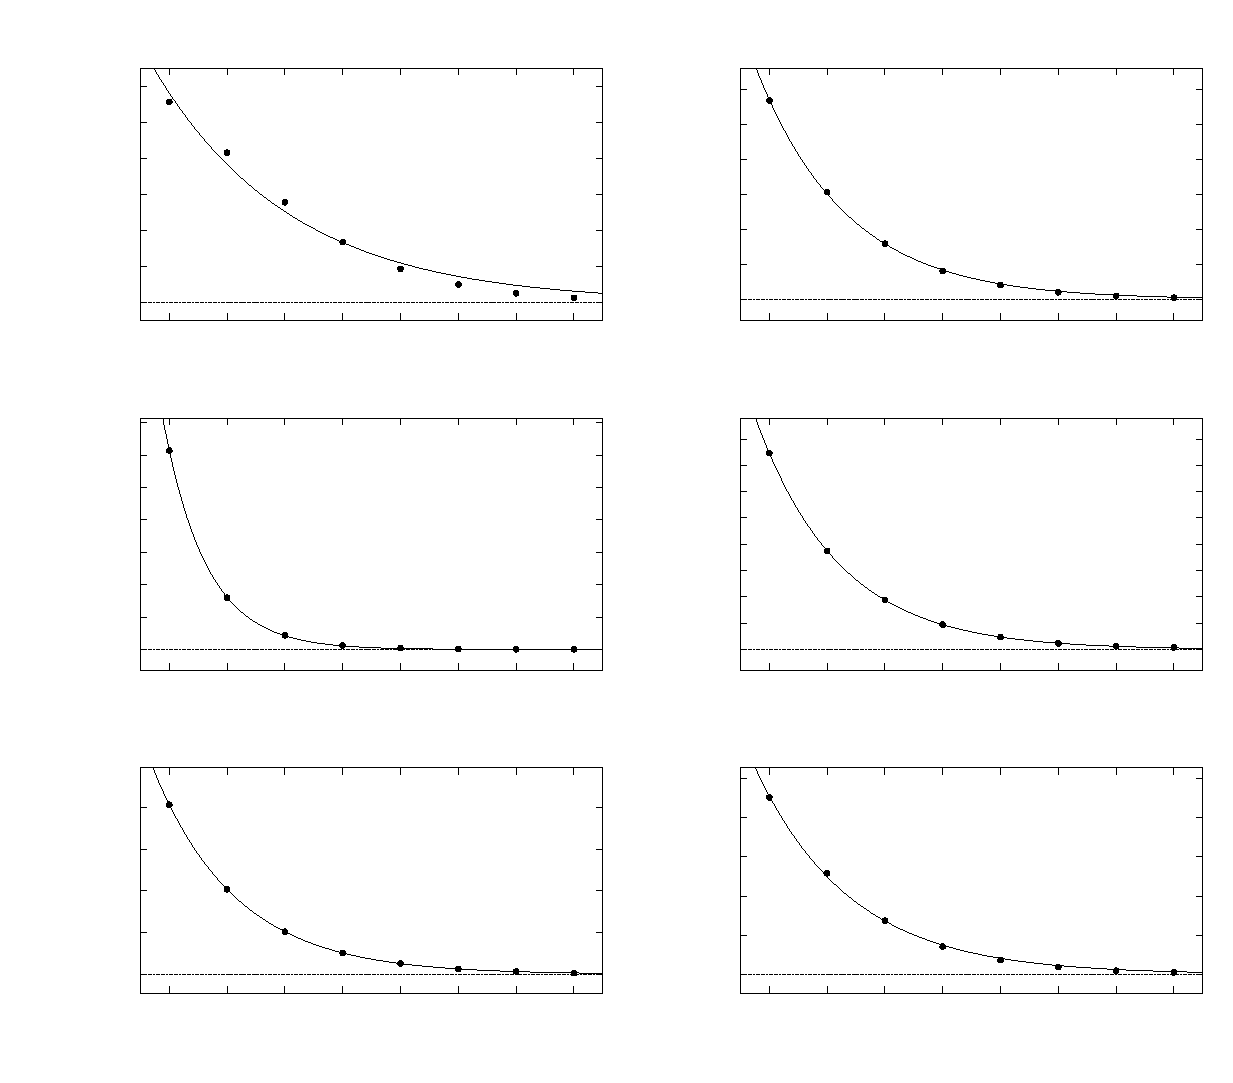
\includegraphics{convergence_tests-inc}}%
    \gplfronttext
  \end{picture}%
\endgroup
\end{document}
